% Created by tikzDevice version 0.10.1 on 2016-12-27 11:53:28
% !TEX encoding = UTF-8 Unicode
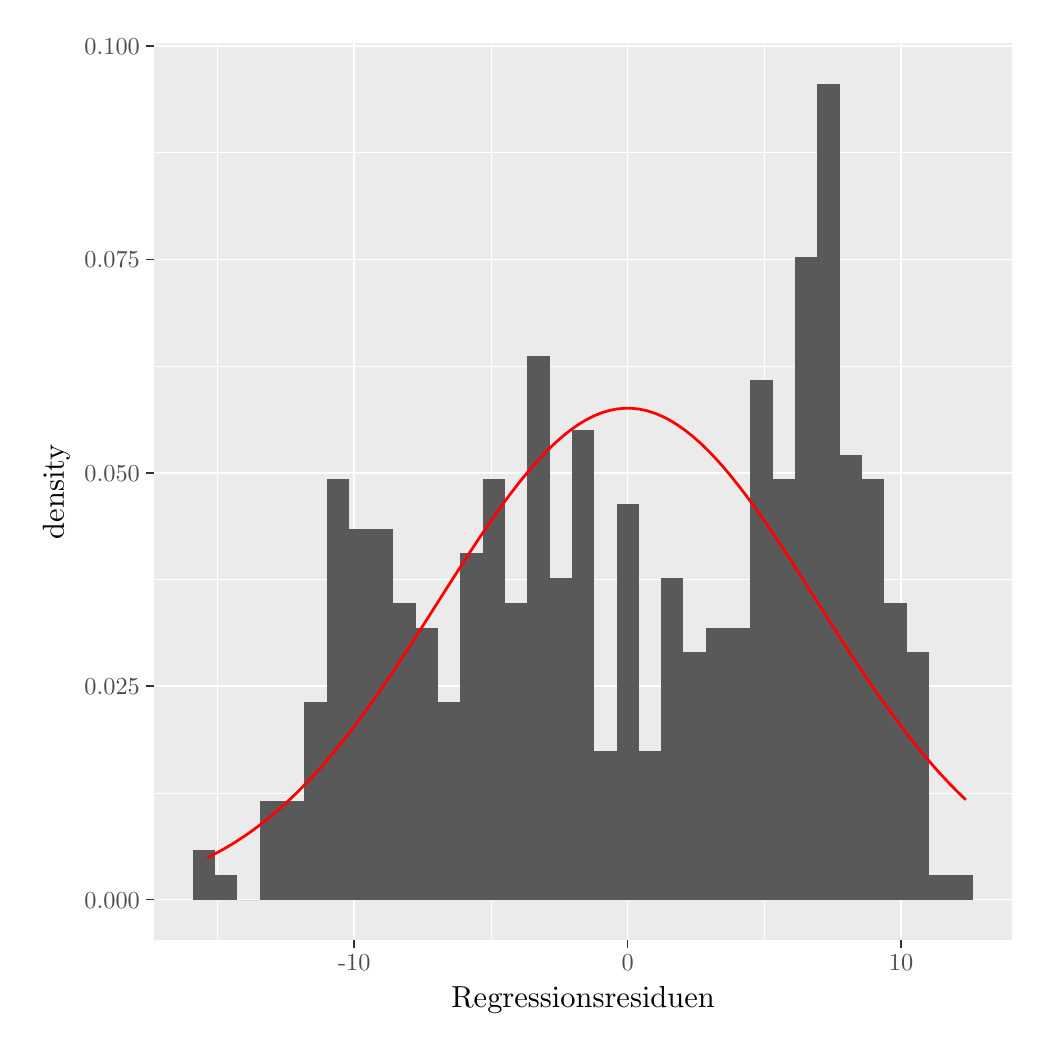
\begin{tikzpicture}[x=1pt,y=1pt]
\definecolor{fillColor}{RGB}{255,255,255}
\path[use as bounding box,fill=fillColor,fill opacity=0.00] (0,0) rectangle (361.35,361.35);
\begin{scope}
\path[clip] (  0.00,  0.00) rectangle (361.35,361.35);
\definecolor{drawColor}{RGB}{255,255,255}
\definecolor{fillColor}{RGB}{255,255,255}

\path[draw=drawColor,line width= 0.6pt,line join=round,line cap=round,fill=fillColor] (  0.00,  0.00) rectangle (361.35,361.35);
\end{scope}
\begin{scope}
\path[clip] ( 45.51, 31.53) rectangle (355.85,355.85);
\definecolor{fillColor}{gray}{0.92}

\path[fill=fillColor] ( 45.51, 31.53) rectangle (355.85,355.85);
\definecolor{drawColor}{RGB}{255,255,255}

\path[draw=drawColor,line width= 0.3pt,line join=round] ( 45.51, 84.82) --
	(355.85, 84.82);

\path[draw=drawColor,line width= 0.3pt,line join=round] ( 45.51,161.91) --
	(355.85,161.91);

\path[draw=drawColor,line width= 0.3pt,line join=round] ( 45.51,239.01) --
	(355.85,239.01);

\path[draw=drawColor,line width= 0.3pt,line join=round] ( 45.51,316.10) --
	(355.85,316.10);

\path[draw=drawColor,line width= 0.3pt,line join=round] ( 68.62, 31.53) --
	( 68.62,355.85);

\path[draw=drawColor,line width= 0.3pt,line join=round] (167.41, 31.53) --
	(167.41,355.85);

\path[draw=drawColor,line width= 0.3pt,line join=round] (266.20, 31.53) --
	(266.20,355.85);

\path[draw=drawColor,line width= 0.6pt,line join=round] ( 45.51, 46.27) --
	(355.85, 46.27);

\path[draw=drawColor,line width= 0.6pt,line join=round] ( 45.51,123.37) --
	(355.85,123.37);

\path[draw=drawColor,line width= 0.6pt,line join=round] ( 45.51,200.46) --
	(355.85,200.46);

\path[draw=drawColor,line width= 0.6pt,line join=round] ( 45.51,277.55) --
	(355.85,277.55);

\path[draw=drawColor,line width= 0.6pt,line join=round] ( 45.51,354.65) --
	(355.85,354.65);

\path[draw=drawColor,line width= 0.6pt,line join=round] (118.01, 31.53) --
	(118.01,355.85);

\path[draw=drawColor,line width= 0.6pt,line join=round] (216.80, 31.53) --
	(216.80,355.85);

\path[draw=drawColor,line width= 0.6pt,line join=round] (315.59, 31.53) --
	(315.59,355.85);
\definecolor{fillColor}{gray}{0.35}

\path[fill=fillColor] ( 59.62, 46.27) rectangle ( 67.68, 64.14);

\path[fill=fillColor] ( 67.68, 46.27) rectangle ( 75.74, 55.21);

\path[fill=fillColor] ( 75.74, 46.27) rectangle ( 83.80, 46.27);

\path[fill=fillColor] ( 83.80, 46.27) rectangle ( 91.86, 82.01);

\path[fill=fillColor] ( 91.86, 46.27) rectangle ( 99.92, 82.01);

\path[fill=fillColor] ( 99.92, 46.27) rectangle (107.98,117.75);

\path[fill=fillColor] (107.98, 46.27) rectangle (116.04,198.16);

\path[fill=fillColor] (116.04, 46.27) rectangle (124.10,180.29);

\path[fill=fillColor] (124.10, 46.27) rectangle (132.16,180.29);

\path[fill=fillColor] (132.16, 46.27) rectangle (140.22,153.49);

\path[fill=fillColor] (140.22, 46.27) rectangle (148.28,144.55);

\path[fill=fillColor] (148.28, 46.27) rectangle (156.35,117.75);

\path[fill=fillColor] (156.35, 46.27) rectangle (164.41,171.35);

\path[fill=fillColor] (164.41, 46.27) rectangle (172.47,198.16);

\path[fill=fillColor] (172.47, 46.27) rectangle (180.53,153.49);

\path[fill=fillColor] (180.53, 46.27) rectangle (188.59,242.83);

\path[fill=fillColor] (188.59, 46.27) rectangle (196.65,162.42);

\path[fill=fillColor] (196.65, 46.27) rectangle (204.71,216.03);

\path[fill=fillColor] (204.71, 46.27) rectangle (212.77, 99.88);

\path[fill=fillColor] (212.77, 46.27) rectangle (220.83,189.22);

\path[fill=fillColor] (220.83, 46.27) rectangle (228.89, 99.88);

\path[fill=fillColor] (228.89, 46.27) rectangle (236.95,162.42);

\path[fill=fillColor] (236.95, 46.27) rectangle (245.01,135.62);

\path[fill=fillColor] (245.01, 46.27) rectangle (253.07,144.55);

\path[fill=fillColor] (253.07, 46.27) rectangle (261.14,144.55);

\path[fill=fillColor] (261.14, 46.27) rectangle (269.20,233.90);

\path[fill=fillColor] (269.20, 46.27) rectangle (277.26,198.16);

\path[fill=fillColor] (277.26, 46.27) rectangle (285.32,278.57);

\path[fill=fillColor] (285.32, 46.27) rectangle (293.38,341.11);

\path[fill=fillColor] (293.38, 46.27) rectangle (301.44,207.09);

\path[fill=fillColor] (301.44, 46.27) rectangle (309.50,198.16);

\path[fill=fillColor] (309.50, 46.27) rectangle (317.56,153.49);

\path[fill=fillColor] (317.56, 46.27) rectangle (325.62,135.62);

\path[fill=fillColor] (325.62, 46.27) rectangle (333.68, 55.21);

\path[fill=fillColor] (333.68, 46.27) rectangle (341.74, 55.21);
\definecolor{drawColor}{RGB}{255,0,0}

\path[draw=drawColor,line width= 1.0pt,line join=round] ( 64.93, 61.41) --
	( 67.67, 62.81) --
	( 70.41, 64.30) --
	( 73.15, 65.89) --
	( 75.89, 67.60) --
	( 78.63, 69.41) --
	( 81.37, 71.34) --
	( 84.11, 73.39) --
	( 86.85, 75.55) --
	( 89.59, 77.84) --
	( 92.33, 80.25) --
	( 95.07, 82.79) --
	( 97.81, 85.45) --
	(100.55, 88.24) --
	(103.30, 91.16) --
	(106.04, 94.20) --
	(108.78, 97.37) --
	(111.52,100.66) --
	(114.26,104.07) --
	(117.00,107.60) --
	(119.74,111.23) --
	(122.48,114.97) --
	(125.22,118.81) --
	(127.96,122.74) --
	(130.70,126.76) --
	(133.44,130.85) --
	(136.18,135.01) --
	(138.92,139.22) --
	(141.66,143.47) --
	(144.41,147.76) --
	(147.15,152.07) --
	(149.89,156.38) --
	(152.63,160.68) --
	(155.37,164.96) --
	(158.11,169.21) --
	(160.85,173.40) --
	(163.59,177.53) --
	(166.33,181.57) --
	(169.07,185.51) --
	(171.81,189.34) --
	(174.55,193.04) --
	(177.29,196.59) --
	(180.03,199.98) --
	(182.77,203.20) --
	(185.52,206.23) --
	(188.26,209.05) --
	(191.00,211.66) --
	(193.74,214.04) --
	(196.48,216.19) --
	(199.22,218.08) --
	(201.96,219.72) --
	(204.70,221.09) --
	(207.44,222.19) --
	(210.18,223.02) --
	(212.92,223.56) --
	(215.66,223.82) --
	(218.40,223.80) --
	(221.14,223.49) --
	(223.88,222.90) --
	(226.63,222.02) --
	(229.37,220.88) --
	(232.11,219.46) --
	(234.85,217.78) --
	(237.59,215.84) --
	(240.33,213.66) --
	(243.07,211.24) --
	(245.81,208.59) --
	(248.55,205.73) --
	(251.29,202.67) --
	(254.03,199.42) --
	(256.77,196.00) --
	(259.51,192.42) --
	(262.25,188.70) --
	(264.99,184.85) --
	(267.74,180.89) --
	(270.48,176.84) --
	(273.22,172.70) --
	(275.96,168.50) --
	(278.70,164.24) --
	(281.44,159.96) --
	(284.18,155.65) --
	(286.92,151.34) --
	(289.66,147.03) --
	(292.40,142.75) --
	(295.14,138.50) --
	(297.88,134.30) --
	(300.62,130.15) --
	(303.36,126.08) --
	(306.10,122.07) --
	(308.85,118.16) --
	(311.59,114.33) --
	(314.33,110.61) --
	(317.07,106.99) --
	(319.81,103.49) --
	(322.55,100.10) --
	(325.29, 96.83) --
	(328.03, 93.68) --
	(330.77, 90.66) --
	(333.51, 87.76) --
	(336.25, 84.99) --
	(338.99, 82.35);
\end{scope}
\begin{scope}
\path[clip] (  0.00,  0.00) rectangle (361.35,361.35);
\definecolor{drawColor}{gray}{0.30}

\node[text=drawColor,anchor=base east,inner sep=0pt, outer sep=0pt, scale=  0.88] at ( 40.56, 43.24) {0.000};

\node[text=drawColor,anchor=base east,inner sep=0pt, outer sep=0pt, scale=  0.88] at ( 40.56,120.34) {0.025};

\node[text=drawColor,anchor=base east,inner sep=0pt, outer sep=0pt, scale=  0.88] at ( 40.56,197.43) {0.050};

\node[text=drawColor,anchor=base east,inner sep=0pt, outer sep=0pt, scale=  0.88] at ( 40.56,274.52) {0.075};

\node[text=drawColor,anchor=base east,inner sep=0pt, outer sep=0pt, scale=  0.88] at ( 40.56,351.62) {0.100};
\end{scope}
\begin{scope}
\path[clip] (  0.00,  0.00) rectangle (361.35,361.35);
\definecolor{drawColor}{gray}{0.20}

\path[draw=drawColor,line width= 0.6pt,line join=round] ( 42.76, 46.27) --
	( 45.51, 46.27);

\path[draw=drawColor,line width= 0.6pt,line join=round] ( 42.76,123.37) --
	( 45.51,123.37);

\path[draw=drawColor,line width= 0.6pt,line join=round] ( 42.76,200.46) --
	( 45.51,200.46);

\path[draw=drawColor,line width= 0.6pt,line join=round] ( 42.76,277.55) --
	( 45.51,277.55);

\path[draw=drawColor,line width= 0.6pt,line join=round] ( 42.76,354.65) --
	( 45.51,354.65);
\end{scope}
\begin{scope}
\path[clip] (  0.00,  0.00) rectangle (361.35,361.35);
\definecolor{drawColor}{gray}{0.20}

\path[draw=drawColor,line width= 0.6pt,line join=round] (118.01, 28.78) --
	(118.01, 31.53);

\path[draw=drawColor,line width= 0.6pt,line join=round] (216.80, 28.78) --
	(216.80, 31.53);

\path[draw=drawColor,line width= 0.6pt,line join=round] (315.59, 28.78) --
	(315.59, 31.53);
\end{scope}
\begin{scope}
\path[clip] (  0.00,  0.00) rectangle (361.35,361.35);
\definecolor{drawColor}{gray}{0.30}

\node[text=drawColor,anchor=base,inner sep=0pt, outer sep=0pt, scale=  0.88] at (118.01, 20.52) {-10};

\node[text=drawColor,anchor=base,inner sep=0pt, outer sep=0pt, scale=  0.88] at (216.80, 20.52) {0};

\node[text=drawColor,anchor=base,inner sep=0pt, outer sep=0pt, scale=  0.88] at (315.59, 20.52) {10};
\end{scope}
\begin{scope}
\path[clip] (  0.00,  0.00) rectangle (361.35,361.35);
\definecolor{drawColor}{RGB}{0,0,0}

\node[text=drawColor,anchor=base,inner sep=0pt, outer sep=0pt, scale=  1.10] at (200.68,  7.44) {Regressionsresiduen};
\end{scope}
\begin{scope}
\path[clip] (  0.00,  0.00) rectangle (361.35,361.35);
\definecolor{drawColor}{RGB}{0,0,0}

\node[text=drawColor,rotate= 90.00,anchor=base,inner sep=0pt, outer sep=0pt, scale=  1.10] at ( 13.08,193.69) {density};
\end{scope}
\end{tikzpicture}
